\newpage
\section{Gestione Profilo}
Il servizio permette ad un utente autenticato di aggiornare e/o modificare i propri dati personali. Cliccando la voce \textit{Gestione Profilo}, presente nella barra a sinistra, il sistema porta l'utente all'interno della pagina dedicata alla gestione del proprio profilo e account. All'interno di questa sezione è possibile:
\begin{itemize}
	\item Inserire un'immagine di profilo;
	\item Modificare il proprio nome;
	\item Modificare il proprio cognome;
	\item Modificare l'email;
	\item Inserire una nuova password.
\end{itemize}

\label{GestioneProfilo}
\begin{figure}[ht]
	\centering
	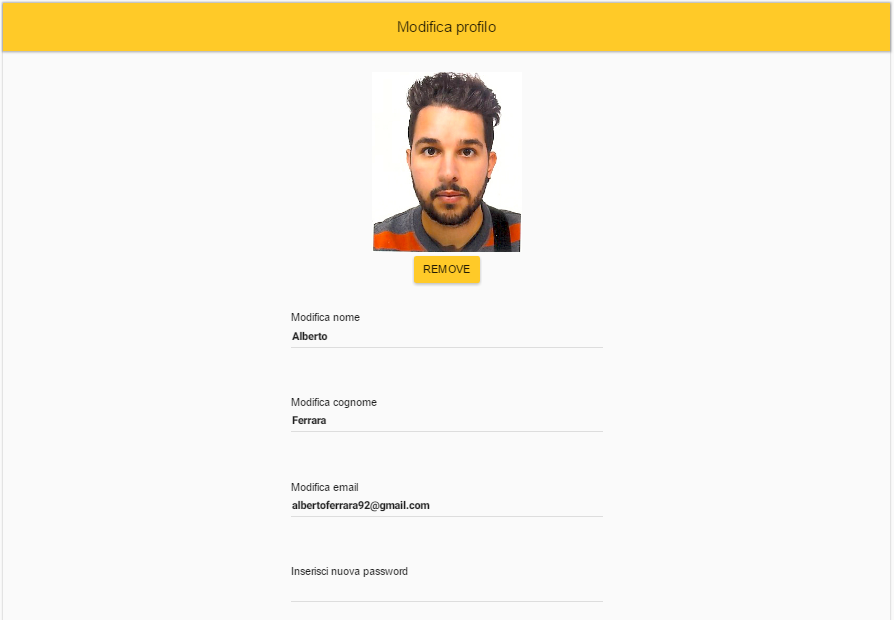
\includegraphics[scale=0.45]{img/gestione_profilo.png}
	\caption{Gestione profilo}
\end{figure}
\FloatBarrier

